\DocumentMetadata{uncompress}  % Aktivuj dekompresi PDF výstupu, která
                               % je potřeba pro správnou funkci balíčku "newpax"% Začátek preambule.
\documentclass{minimal}
\usepackage[resetfonts]{cmap}
\usepackage{lmodern}
\usepackage[czech]{babel}
\usepackage[utf8]{inputenc}
\usepackage[T1]{fontenc}
\usepackage[linktodoc]{pdfpages}
\usepackage{imakeidx}
% \directlua{require("newpax")}  % Načti luový modul "newpax"
\usepackage{newpax}          
\newpaxsetup{usefileattributes}
\usepackage[pdfusetitle]{hyperref}

\begin{document}
% fit index onto the last page (maybe templatesize)
% also fix links
% \directlua{newpax.writenewpax("main")}

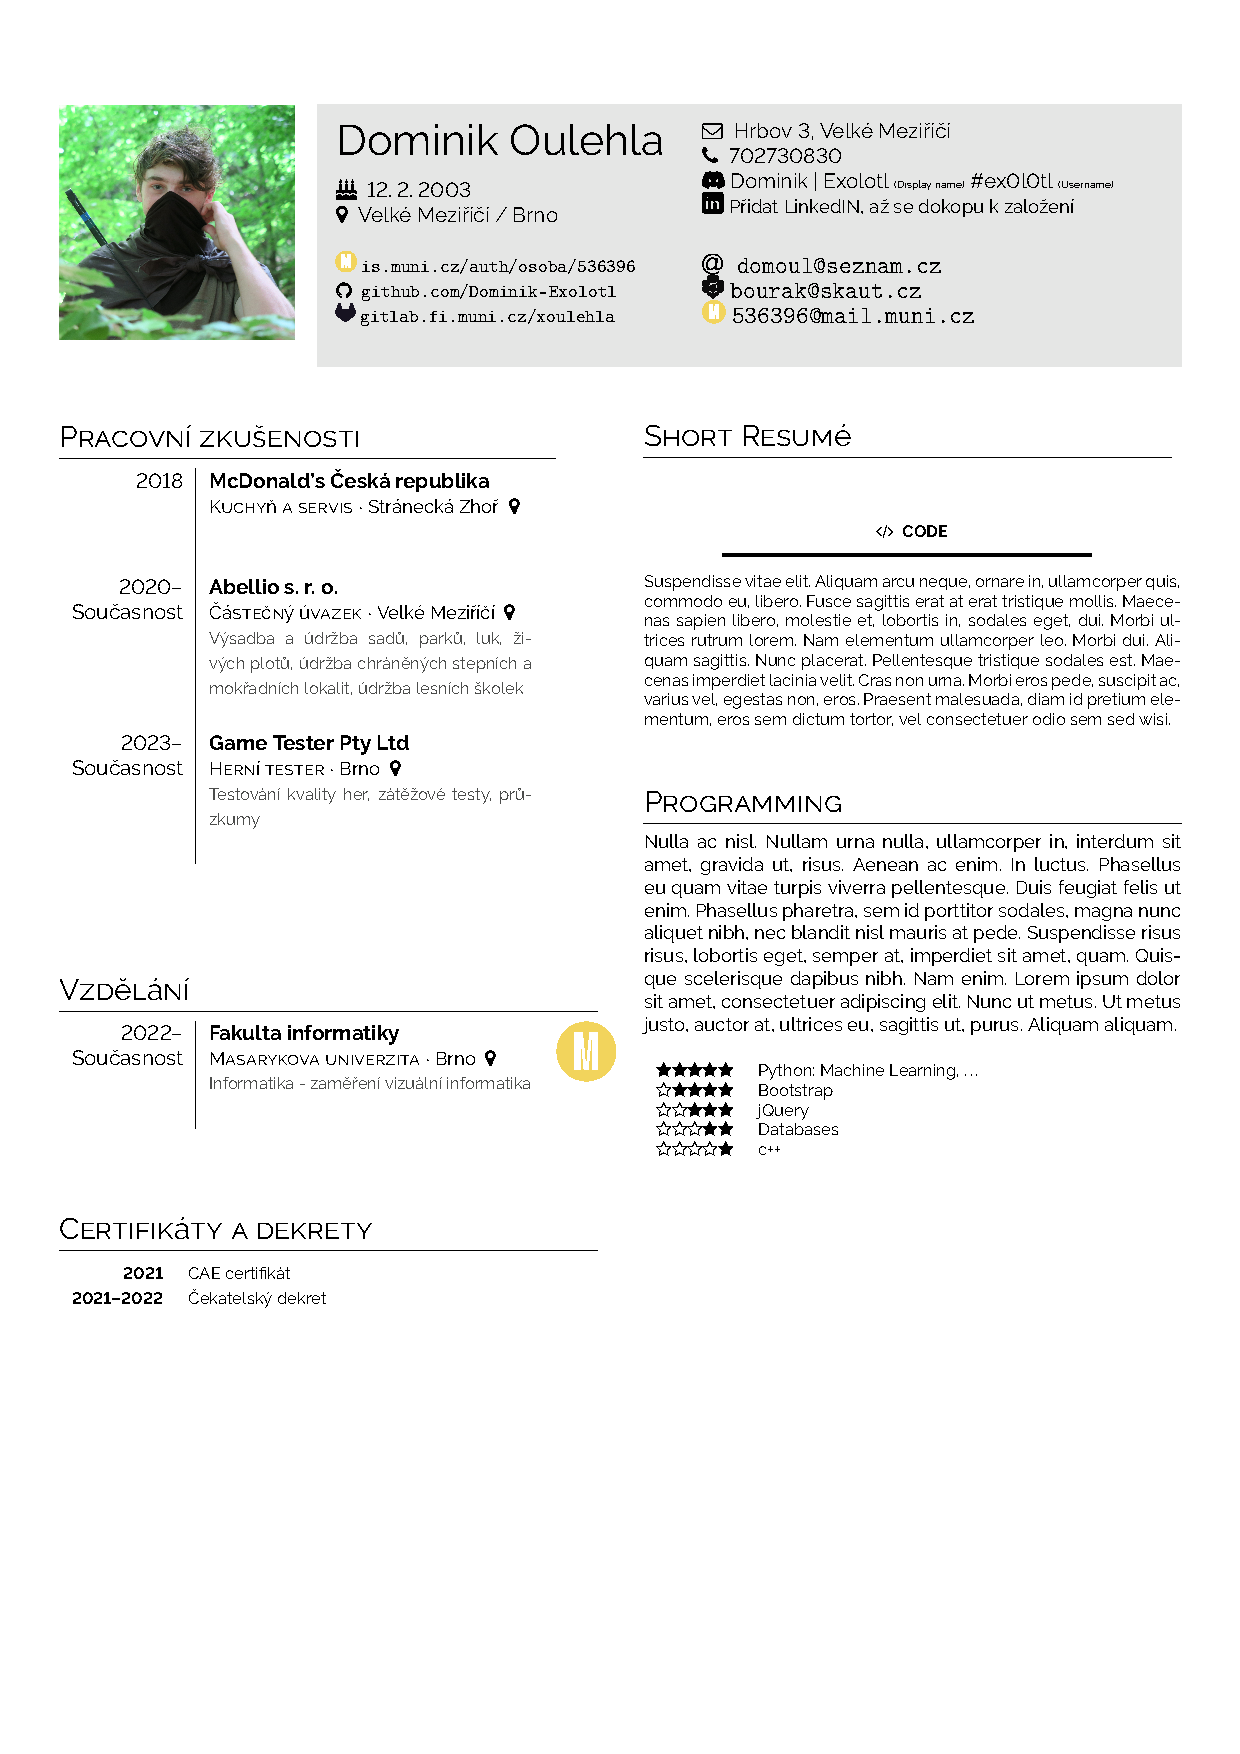
\includepdf[pages=-]{main.pdf}

\directlua{newpax.writenewpax("finals_thesis")}
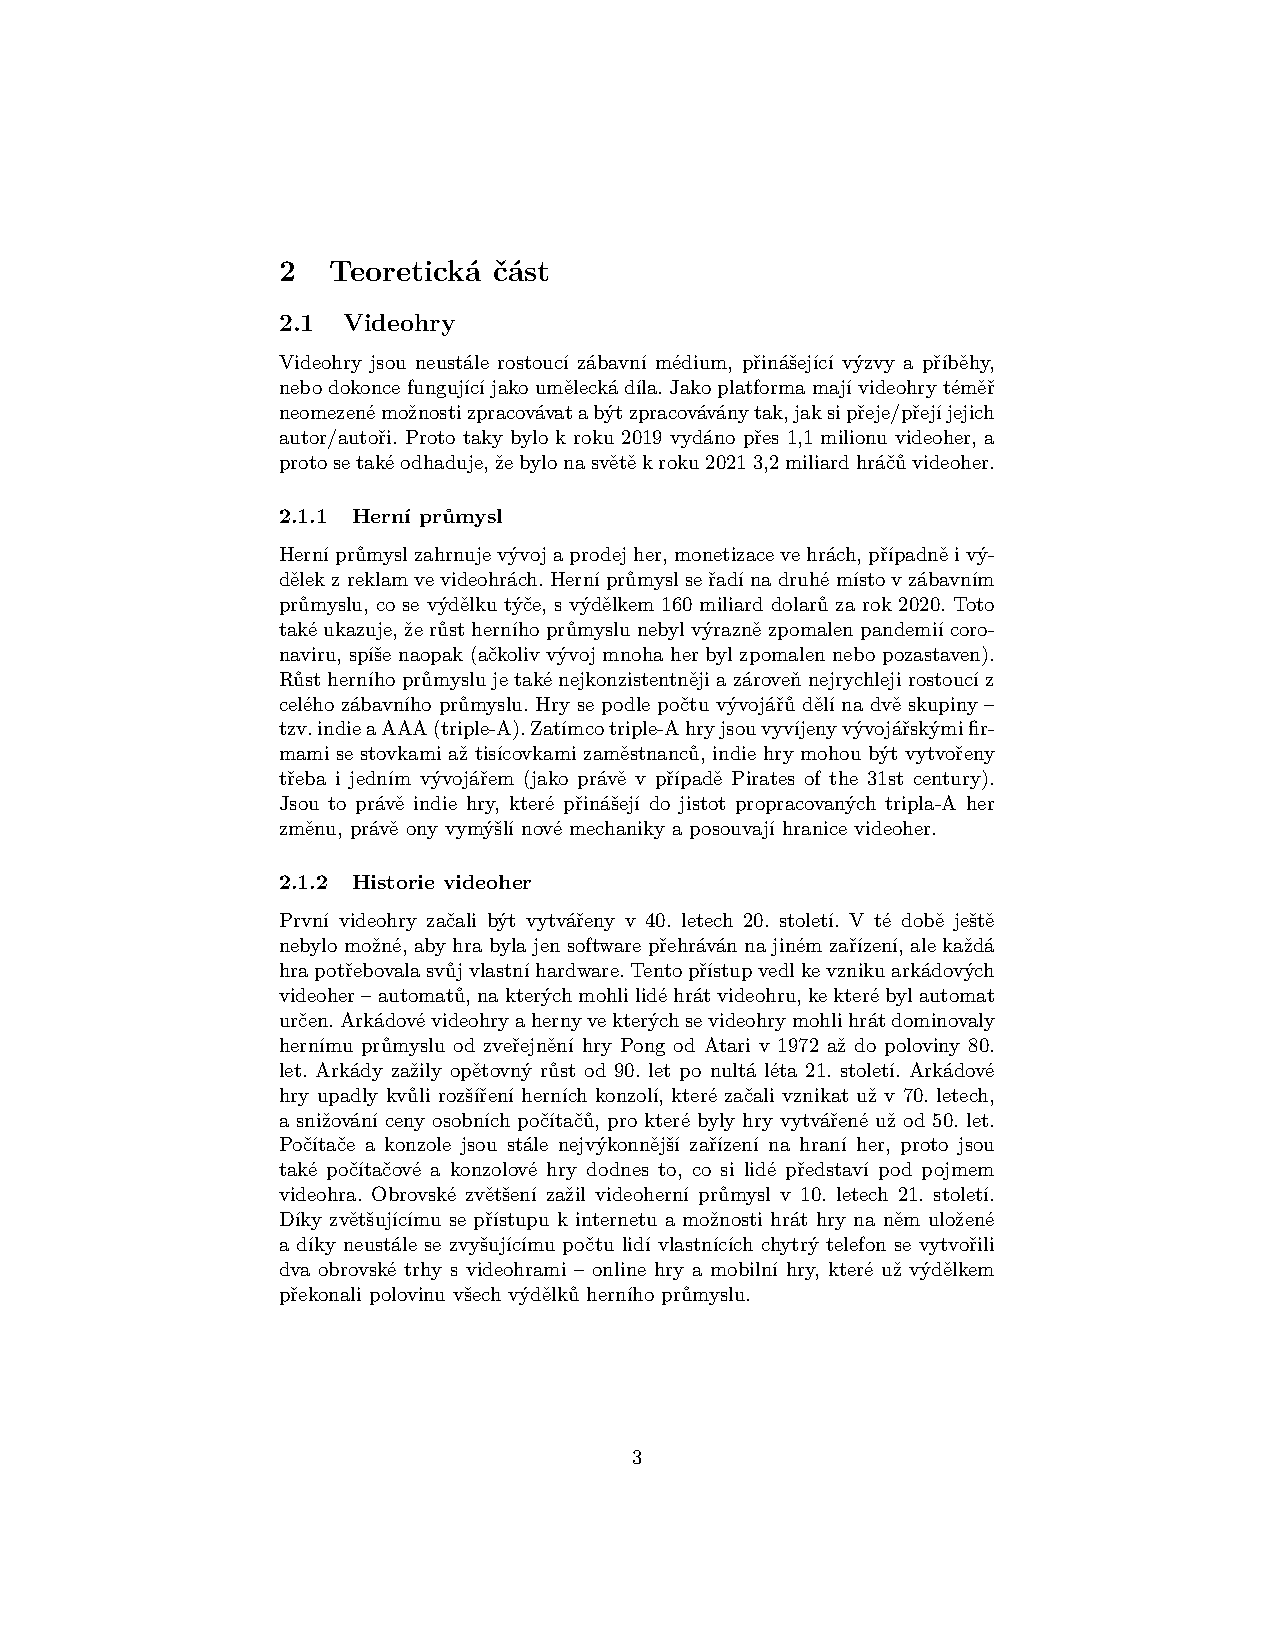
\includepdf[pages=1-3]{finals_thesis.pdf}
\end{document}